
\documentclass[extendedabs]{AAVL}

\runninghead{Claus, Fitzgibbon}{Plumbline Constraint for the RF Model}

\begin{document}

\title{Numerical simulations for selected 1D and 2D Mass-spring
models and Applications}

\addauthor{Sachin Chandrasekara}{SC/2018/10559}{1}


\addinstitution{
Department of Mathematics,\\
Faculty of Science,\\
University of Ruhuna}

\maketitle
\section{Background}

\noindent

One of the approaches used for modelling of the musculoskeletal system during locomotion is the so-called mass–spring–damper (MSD) modelling
approach. In this method, a small number of masses reflect the inertia properties of the various segments of the human body, namely hard tissues and soft tissues. Springs and dampers reflect the mechanical properties of the various segments, including bones, muscles, tendons and ligaments. These relatively simple models of the human body are very useful for learning the basic concepts of locomotion. Therefore, MSD models have therefore been widely used to explain various aspects of locomotion, including the mechanics of running and jumping and filling the human body during these activities.\\

This project is concerned only with running and hopping. In addition, the main focus is on the MSD models themselves and not on the findings obtained from these models. The models tested include single-body and multi-body models as well as passive and active models. When we comes to the passive models, many of the MSD models that have been formed so far belong to this category. And also passive models may be classified as either one-body or multi-body models depending on the number of their masses. 
\subsection{One-body models}
The human’s muscle skeletal system can be considered mechanically as an actively-driven, nonlinear, multi component spring-mass system. Here it is presumed that it actually acts like a point mass bouncing passively on a mass less spring without viscous losses. This is the simplest model possible for any bouncing system where we can find in our human body. The model provides important insights and describes
interdependence of parameters that characterise running and hopping. 
\begin{itemize}
    \item one-dimensional (1D) motion model (Fig. 1(a))
used for in-place hopping when there is no forward motion.
    \item two-dimensional (2D) motion model (Fig. 1(b))
used to study in-plane forward running.
\end{itemize}

One body models are potentially the most frequently used MSD models. They are used for various purposes, but the most main applications of single-body mass-spring models is, perhaps, the determination of low-extremity stiffness and the prediction of ground reaction force (GRF) during hopping and running. 

\begin{figure}[hbt!]
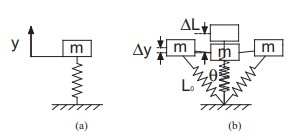
\includegraphics[width=\linewidth]{images/a.jpg}
\caption{Schematic representation of the (a) 1D motion
and (b) 2D motion passive one-body mass–spring models body}
\vspace{-2mm}
\label{fig:a}
\end{figure}

Considering the significance of one-body models for the determination of body stiffness, this application of one-body models is demonstrated in the present study. You can see in \cite{a} used the 1D motion model (hopping model) for prediction of the vertical stiffness and force of the human body in in place hopping. And also in a more recent study \cite{b}, the 2D motion model was recruited to calculate the vertical
and leg stiffness during running. 

\section{Approach}
The vertical stiffness is defined as the ratio of the vertical leg spring compression to peak vertical Ground Reaction Force (GRF) at the middle of the stance phase \cite{b,c}. And also \cite{d} analyzed available methods for the measurement of vertical and leg stiffness using single-body mass–spring models. 

\subsection{Equations of motion}
\label{a}
The equation of motion for a 1D (hopping) motion model figure \ref{fig:a} (a) can be written as follows.

\begin{equation}
        m \Ddot{y} + k_{ver}y = mg
\end{equation}
where $k_{ver}$ is the vertical stiffness and is calculated
as,
\begin{equation}
\label{b}
    k_{leg} = \frac{F_{max}}{\Delta y_{max}}
\end{equation}
where $F_{max}$ is the maximum vertical force and $\Delta y_{max}$
is the maximum spring deformation. 
For the 2D (running model) motion model, the equation of motion may be written as follows,

\begin{equation}
        m \Ddot{y} + k_{leg}y = mg
\end{equation}
where $k_{leg}$ is the leg stiffness and is calculated as.
\begin{equation}
    k_{leg} = \frac{F_{max}}{\Delta L}
\end{equation}
where $F_{max}$ is the maximum vertical force and $\Delta L$ is the vertical displacement of the mass that is formulated as,
\begin{equation}
    \Delta L = \Delta y + L_0(1-\cos{\theta})
\end{equation}
where $L_{0}$ is the standing leg length and the angle $\theta$ is calculated as follows,
\begin{equation}
  \theta = \sin^{-1}\frac{\Dot{x}t_{c}}{2L_{0}}
\end{equation}
where $\Dot{x}$ is the forward speed and $t_{c}$ is the contact time with the ground.

\subsection{Calculation of vertical and leg stiffness}
The simplest method is proposed by McMahon and Cheng \cite{e} and was presented in section \ref{a} equation \eqref{b}. And the vertical displacement can be calculated by integrating the vertical acceleration data. And also the vertical stiffness can be calculated as corresponding to reference \cite{f}. 
  
\section{Reference}
\begin{thebibliography}{}
\bibitem{a}
  Farley, C. T.,\ Blickhan. R,\  Saito.j\ \& Beeman, D.\ (1991) {\it  Hopping frequency in humans: a test of how springs set stride frequency in bouncing gaits}.
  
\bibitem{b}
Hobara, H.,\ Inoue, K.,\ Gomi, K.,\ Sakamoto, M.,Muraoka, \ \& Kanosue, K. {\it Continuous change in spring–mass characteristics during a 400 m sprint. J. Sci. Med. Sport, 2009,}

\bibitem{c}
Blickhan. R. {\it The spring–mass model for running and hopping. J. Biomech., 1989}, {22(11–12), 1217–1227.} 

\bibitem{d}
Butler, R. J., \ Crowell, H. P.,\ \& Davis, I. M. {\it  Lower extremity stiffness: implications for performance and injury. Clin. Biomech., 2003}, { 18(6), 511–517.}

\bibitem{e}
McMahon, T. A. ,\ \& Cheng, G. C.  {\it The mechanics
of running: how does stiffness couple with speed? J. Biomech., 1990, 
}{23},{ 65–78.}

\bibitem{f}
McMahon, T. A., Valiant, G., \ \&Frederick, E. C. {\it Groucho running. J. Appl. Physiol.}, {1987, 62(6),2326–2337}.

\end{thebibliography}

\end{document}
